\documentclass[12pt, a4paper,reqno]{article}

\usepackage{amsmath}
\usepackage{amssymb}
\usepackage{graphicx}
\usepackage{float}
\usepackage{caption}
\usepackage{subcaption}
\usepackage{pdfpages}
\usepackage{minted}
\usepackage{color, soul}

\setlength{\parindent}{0pt}
\setlength{\parskip}{1em}


%
% Begin Document
%
\begin{document}

% TODO: Add date
% Cover Page

\includepdf[pages=-]{End_Assessment_Front_Page_HYXC3.pdf}


%
% Question 1
%
\section*{Question 1}

% Subsection 1(a)
\subsection*{1(a)}
With reference to the diagram of the basic \emph{logistic unit} on the following page:

The input vector $\mathbf{x}$ is the input to the \emph{logistic unit}.

Each input ${x}_i$ has an associated weight $\theta_i$. The weights are set to a random value prior to \emph{training}. The \emph{training} process determines these weights.

The product of each input $x_i$ and weight $\theta_i$ is summed to produce a weighted sum $z$.

The non-linear activation function $a$ then acts upon $z$ to produce the \emph{logisitc unit} output $h_\theta(x)$, $h_\theta(x) = a(z)$.

% Subsection 1(b)
\subsection*{1(b)}

Consider the diagram of Question 1(a).

The weighted sum of the inputs, $z$, is:

\begin{equation}
z = \sum_{j=1}^{n}\theta_j x_j = \theta^T x
\end{equation}

where $x_i$ is the $i^{th}$ element of input vector $\mathbf{x}$ of length $n$, and $\theta_i$ is the associated \emph{weight}. 

And, the output from the \emph{logistic unit}, $h_\theta(x)$, is:

\begin{equation}
h_\theta(x) = a(z)
\end{equation}

where $a$ is a non-linear \emph{activation function}.

% Subsection 1(a) - diagram
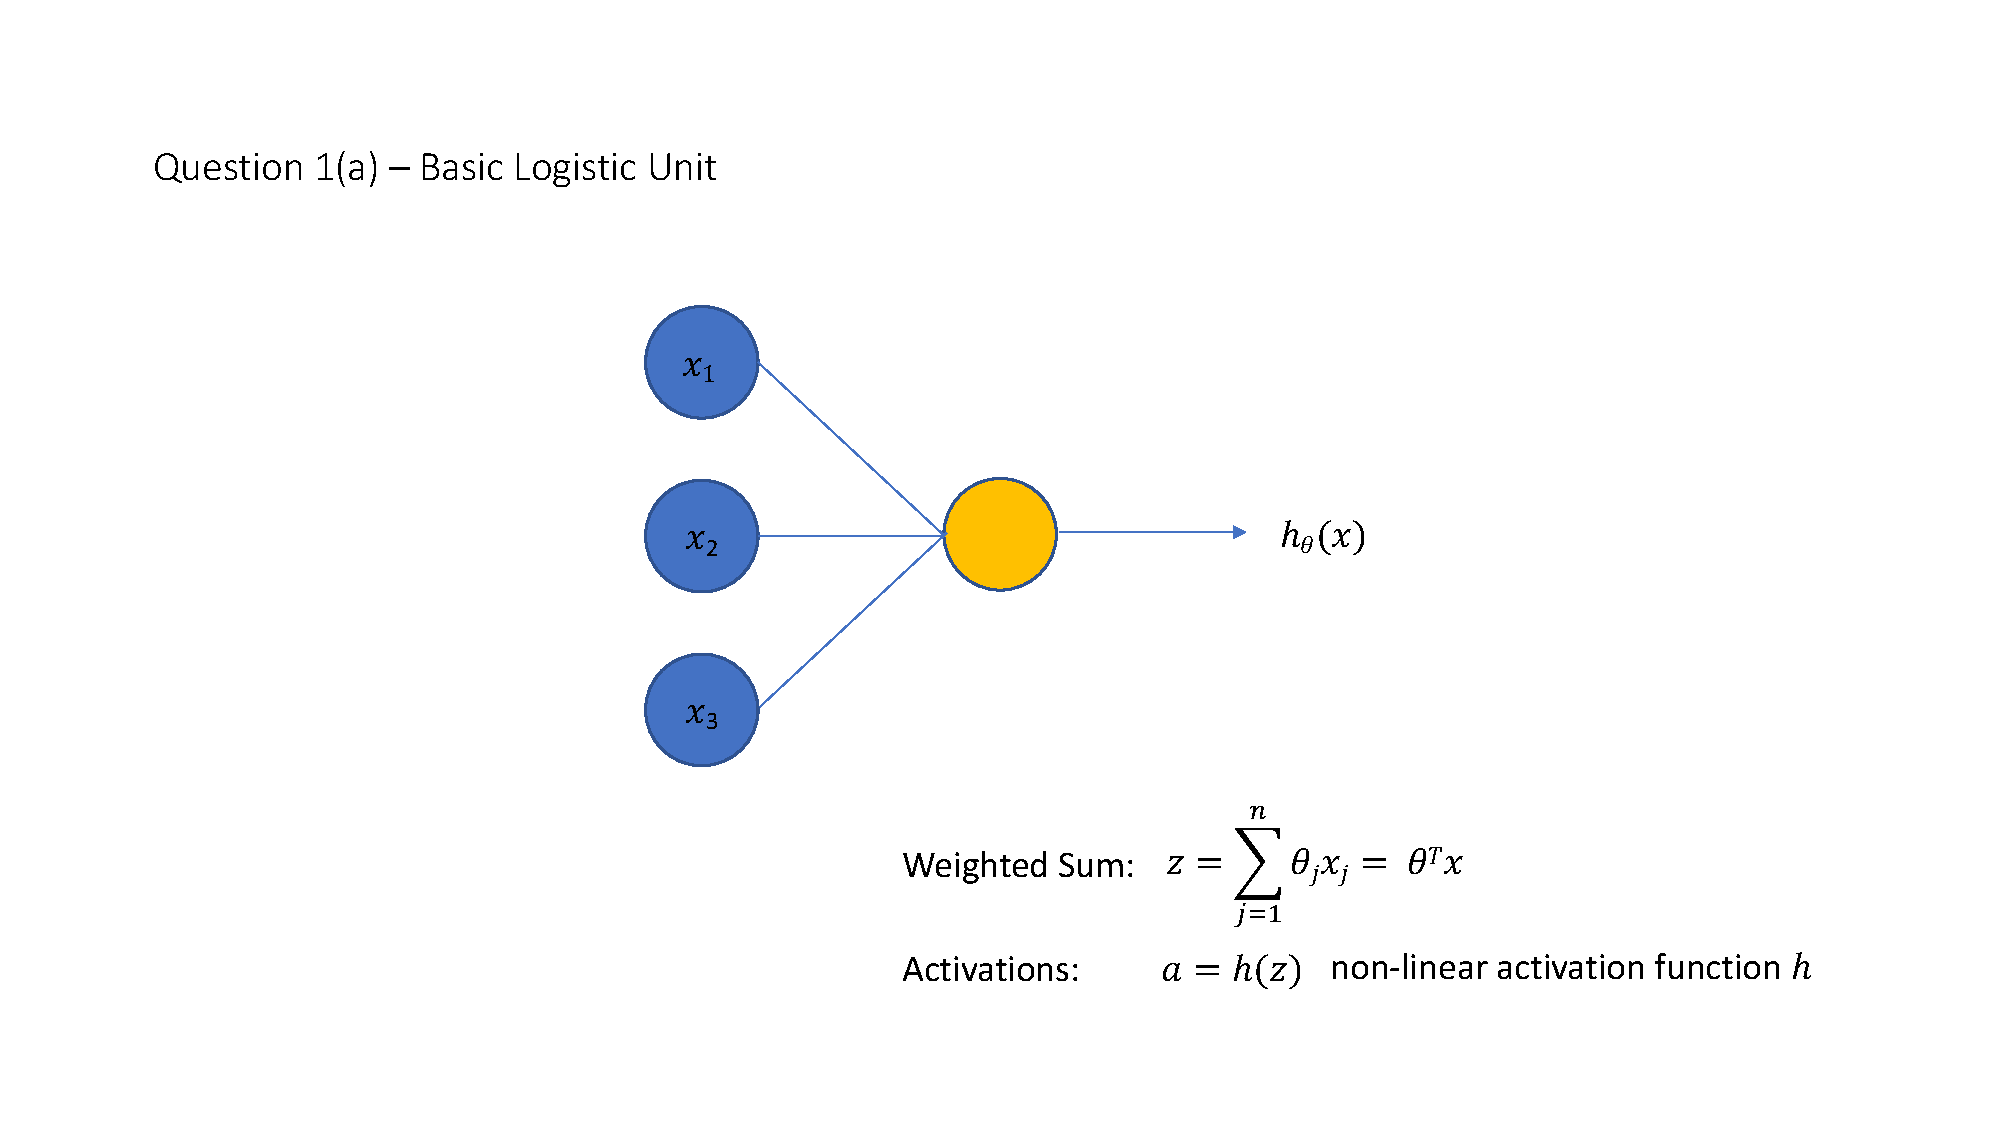
\includepdf[angle=+90]{question_1a.pdf}

% Subsection 1(c)
\subsection*{1(c)}
See diagram on following page.

% Subsection 1(d)
\subsection*{1(d)}
Consider the diagram of Question 1(c):



% Subsection 1(c) - diagram
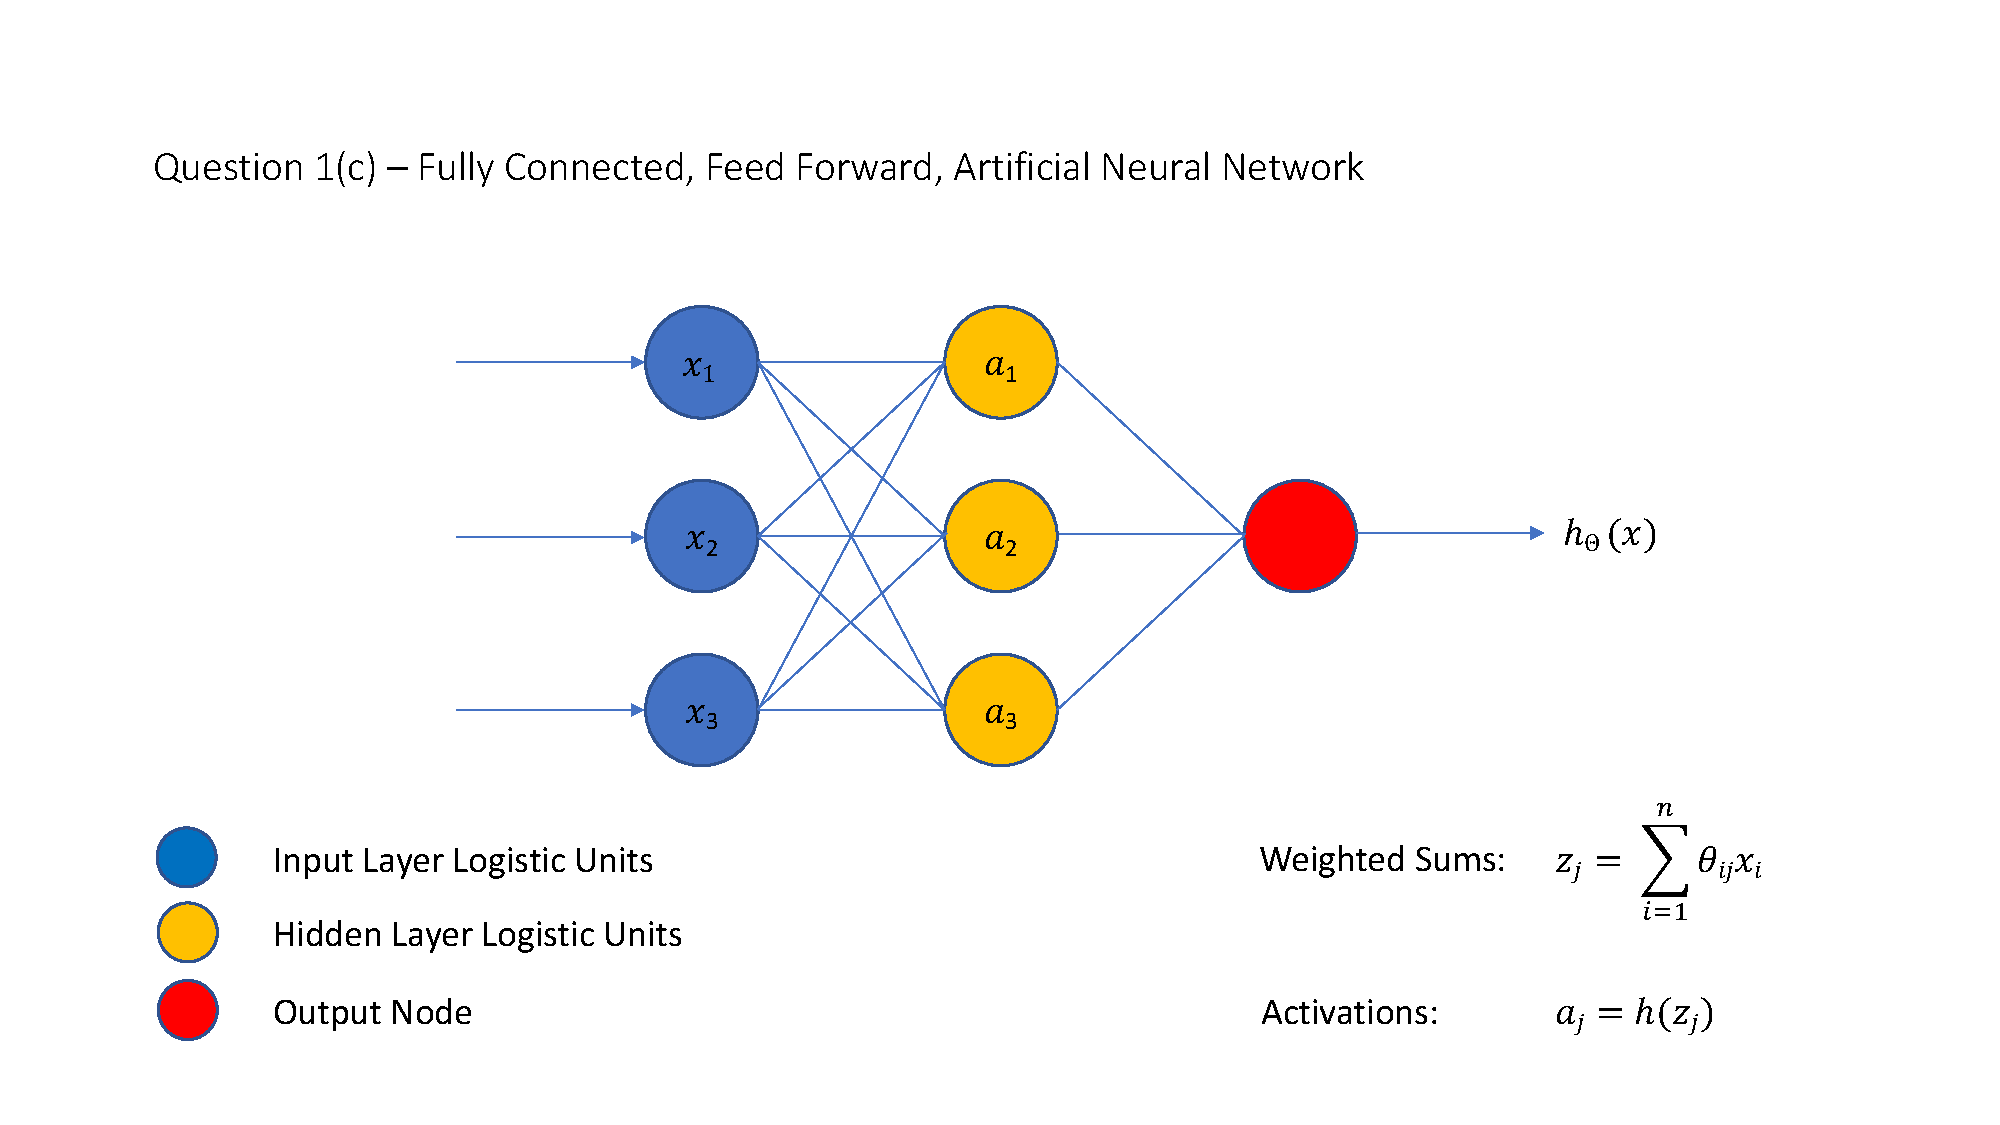
\includepdf[angle=+90]{question_1c.pdf}

% Subsection 1(e)
\subsection*{1(e)}
\hl{TODO}

% Subsection 1(f)
\subsection*{1(f)}
Artificial Neural Networks (ANNs) are described as \emph{shallow} or \emph{deep}, and \emph{wide} or \emph{narrow}. \emph{shallow} or \emph{deep} refers to the number of layers in the network, and \emph{wide} or \emph{narrow} refers to the number of nodes in each layer.

The \emph{credit assignment path}, the CAP, of a neural network is a measure of the number of data transformations that occur as data passes through the network. For \emph{feed-forward} networks the CAP is the number of \emph{hidden layers} plus one.

A \emph{deep} neural network is generally considered to be a network with multiple layers and a CAP $>$ 2.

% Subsection 1(g)
\subsection*{1(g)}
\hl{TODO}


%
% Question 2
%
\clearpage\section*{Question 2}

\subsection*{2(a)}
\hl{TODO}

\subsection*{2(b)}
\hl{TODO}

\subsection*{2(c)}
\hl{TODO}

\subsection*{2(d)}
\hl{TODO}

\subsection*{2(e)}
\hl{TODO}

\subsection*{2(f)}
\hl{TODO}

\subsection*{2(g)}
\hl{TODO}

\subsection*{2(h)}
\hl{TODO}


%
% Question 3
%
\clearpage\section*{Question 3}

\subsection*{3(a)}
\hl{TODO}

\subsection*{3(b)}
\hl{TODO}

\subsection*{3(c)}
\hl{TODO}

\subsection*{3(d)}
\hl{TODO}

\subsection*{3(e)}
\hl{TODO}

\subsection*{3(f)}
\hl{TODO}


%
% Question 4
%
\clearpage\section*{Question 4}

\subsection*{4(a)}
\hl{TODO}

\subsection*{4(b)}
\hl{TODO}

\subsection*{4(c)}
\hl{TODO}

\subsection*{4(d)}
\hl{TODO}

\subsection*{4(e)}
\hl{TODO}

\subsection*{4(f)}
\hl{TODO}

\begin{listing}
\inputminted[linenos]{python}{question_4f.py}
\caption{Question 4f}
\end{listing}

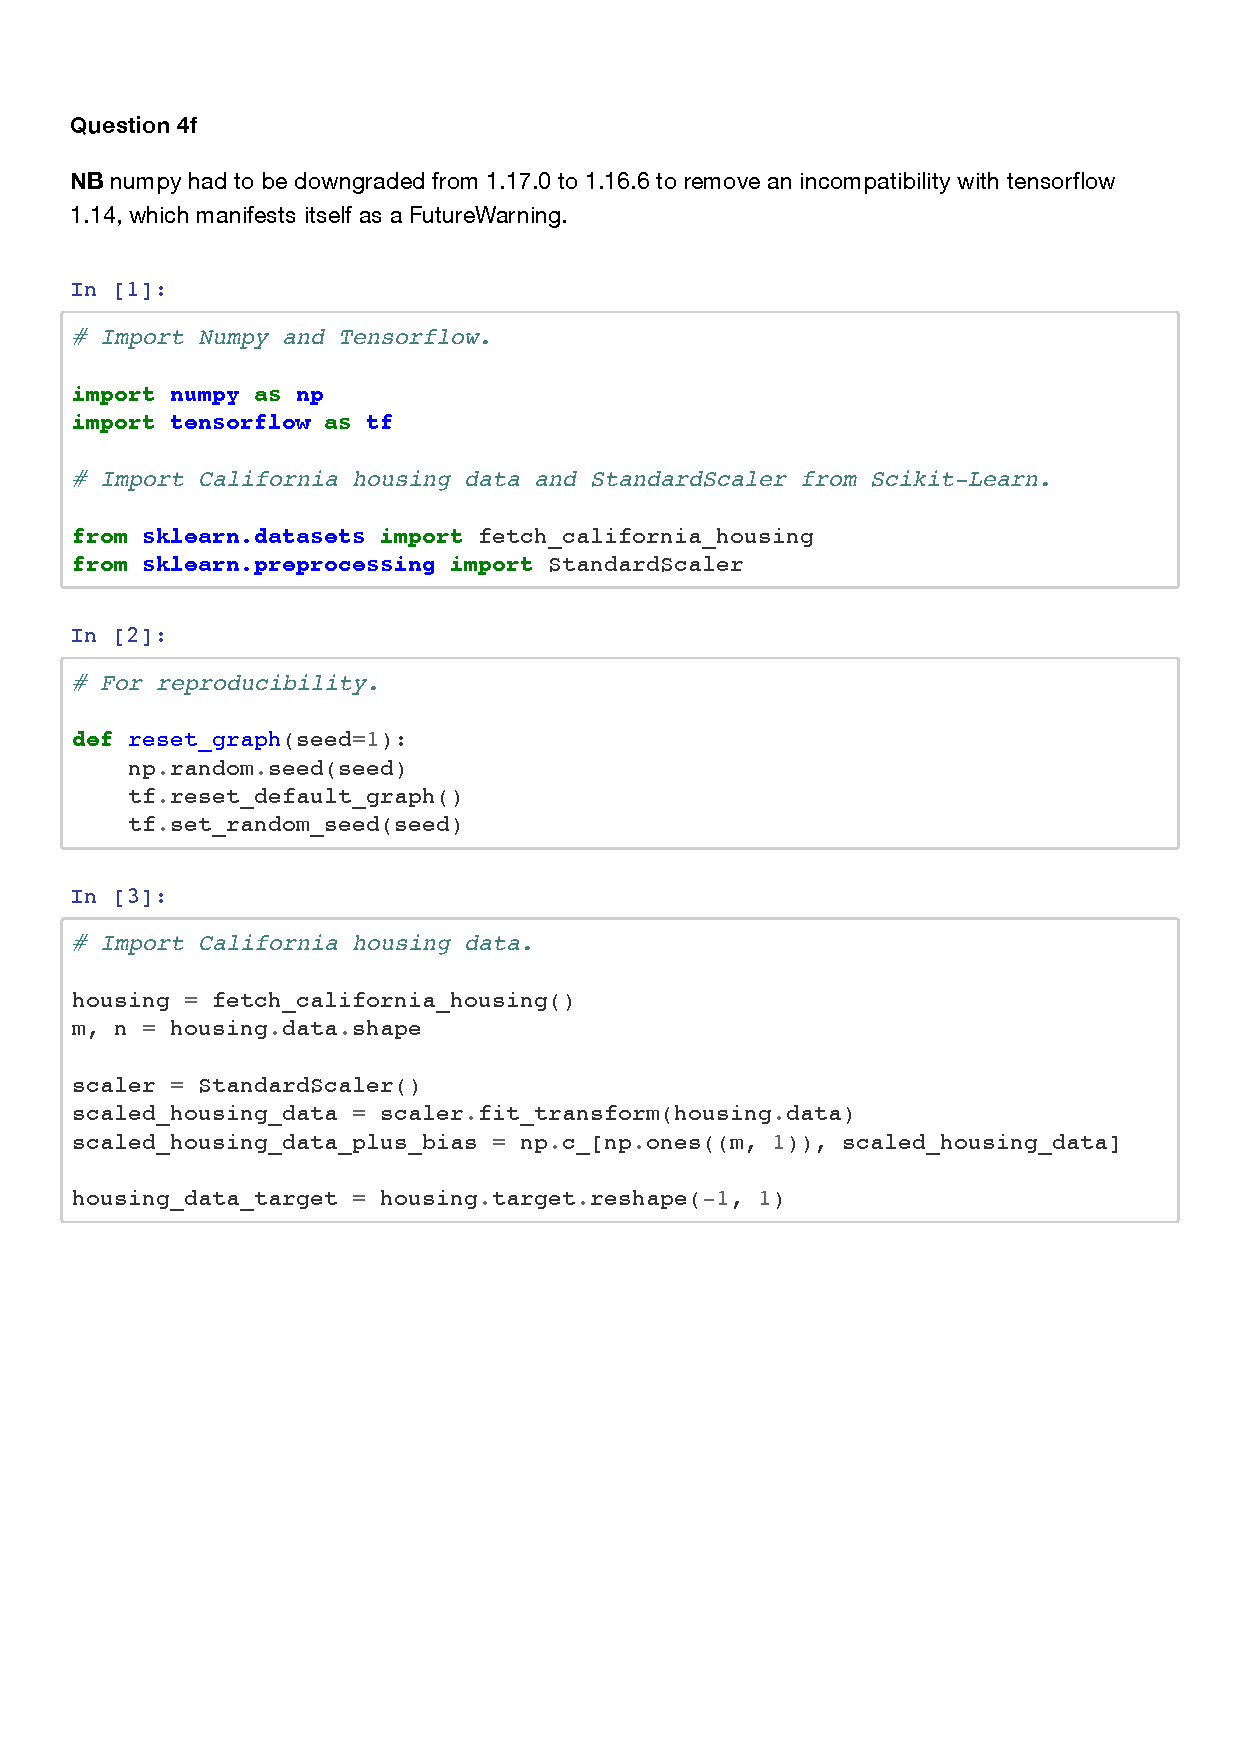
\includepdf[pages=-]{question_4f.pdf}

%
% Question 5
%
\clearpage\section*{Question 5}

\subsection*{5(a)}
\hl{TODO}

\subsection*{5(b)}
\hl{TODO}

\subsection*{5(c)}
\hl{TODO}

\subsection*{5(d)}
\hl{TODO}

\subsection*{5(e)}
\hl{TODO}

\subsection*{5(f)}
\hl{TODO}


\end{document}
